\documentclass[14pt]{report}

\usepackage{geometry}
\usepackage[utf8]{inputenc}
\usepackage{amsmath}
\usepackage{amsfonts}
\usepackage{amssymb}
\usepackage{graphicx}
\usepackage[utf8]{inputenc}
\usepackage{amsmath}
\usepackage{amsfonts}
\usepackage{amssymb}
\usepackage[shortlabels]{enumitem}
\usepackage{listings}
\usepackage{xcolor}
\usepackage[most]{tcolorbox}
\usepackage{mathtools}
\usepackage{float}
\usepackage[colorlinks=false, linktocpage=true]{hyperref}
\usepackage{enumitem}

\usepackage{booktabs}% http://ctan.org/pkg/booktabs
\newcommand{\tabitem}{~~\llap{\textbullet}~~}
\usepackage{longtable}
 
\usepackage{caption}
\DeclareCaptionType{code}[Code Listing][List of Code Listings] 

\definecolor{codegreen}{rgb}{0,0.6,0}
\definecolor{codegray}{rgb}{0.5,0.5,0.5}
\definecolor{codepurple}{rgb}{0.58,0,0.82}
\definecolor{backcolour}{rgb}{0.95,0.95,0.92}
 
\lstdefinestyle{mystyle}{
    backgroundcolor=\color{backcolour},   
    commentstyle=\color{codegreen},
    keywordstyle=\color{magenta},
    numberstyle=\tiny\color{codegray},
    stringstyle=\color{codepurple},
    basicstyle=\ttfamily\footnotesize,
    breakatwhitespace=false,         
    breaklines=true,                 
    captionpos=b,                    
    keepspaces=true,                 
    numbers=left,                    
    numbersep=5pt,                  
    showspaces=false,                
    showstringspaces=false,
    showtabs=false,                  
    tabsize=2
}
 
\lstset{style=mystyle}

\setlength{\parindent}{0em}
\setlength{\parskip}{1em}

\author{Brian Rashap, Ph.D.}
\title{PHYS 1320 - Calculus-based Physics II}

\geometry{letterpaper, portrait, margin=0.75in}

\begin{document}

\begin{center}
\textbf{Physics 1320 - Calculus-based Physics II \\ Summer 2022 \\ Midterm Exam I}
\end{center}

\textbf{Question 1} (20 pts)

Consider the following configuration:

\begin{figure}[H]
\begin{center}
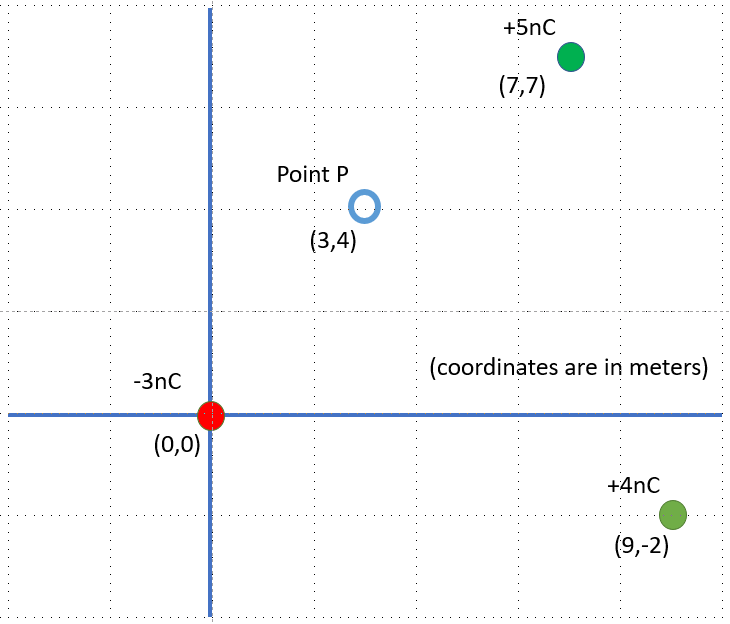
\includegraphics[scale=0.30]{exam1_1.png}
\end{center}
\end{figure}
\begin{enumerate}[label=\Alph*]
\item Draw the electric field lines that result from the three charges.
\item What is the total Electric Field at point P expressed in vector notation (i.e., $\vec{E} = E_x \hat{i} + E_y \hat{j}$)?
\item What is the magnitude ($E$) and direction ($\theta$) of the Electric Field $\vec{E}$?
\item If an electron is placed at point P, what Force ($\vec{F}$) will it experience?
\end{enumerate}

\textbf{Question 2} (15 pts)

Consider a ring of charge on the xy-plane with a radius $R = 10cm$. 

\begin{figure}[H]
\begin{center}
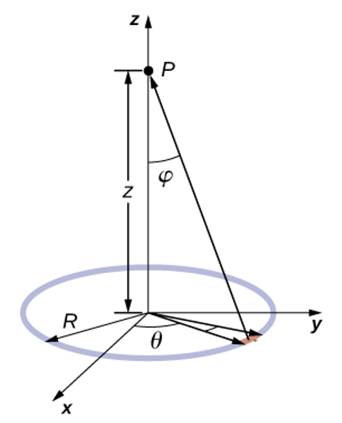
\includegraphics[scale=0.40]{exam1_2.png}
\end{center}
\end{figure}

If the total charge on the ring is $-31.5 \mu C$. 

\begin{enumerate}[label=\Alph*]
\item What is the charge density on the ring?
\item From the charge density, calculate the electric field ($\vec{E}$) at point P where z = 5cm.
\end{enumerate}

\newpage
\textbf{Question 3} (15 pts)

Consider the following surface (dimensions are in cm). 

\begin{figure}[H]
\begin{center}
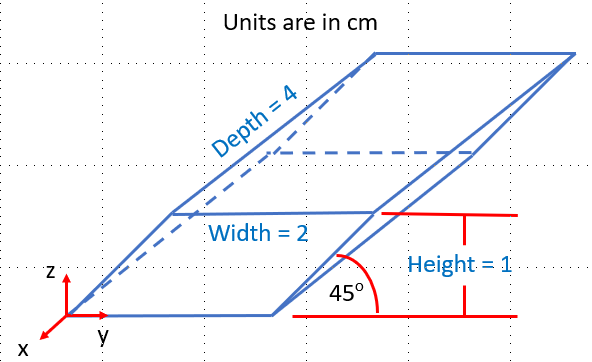
\includegraphics[scale=0.40]{exam1_4.png}
\end{center}
\end{figure}
Assume that there is a uniform electric field of $\vec{E} = E_x (-\hat{i}) + E_y \hat{j}$, where $E_x = 3 \frac{N}{C} $ and $E_y = 8 \frac{N}{C}$. Calculate the Flux through:

\begin{enumerate}[label=\Alph*]
\item Front surface?
\item Top surface?
\item Right surface?
\item Net flux through all surfaces combined?
\end{enumerate}

\textbf{Question 4} (15 pts)

Consider the following hallow, spherical, conducting shell. 

\begin{figure}[H]
\begin{center}
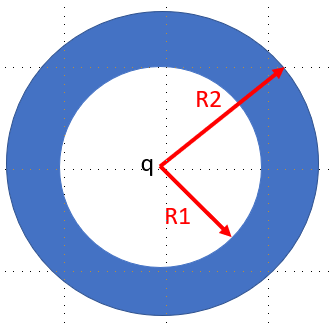
\includegraphics[scale=0.40]{exam1_5.png}
\end{center}
\end{figure}
Assume the total charge on the sphere is $Q_o = 60nC$, and that there is a charge of $Q_{center} = 45nC$ at the center. For the case where $R1 = 0.25m$ and $R2 = 0.42m$. Using Gauss's Law, find:

\begin{enumerate}[label=\Alph*]
\item The electric field ($\vec{E}$) at a point in the hallow cavity at a distance 0.20m from the center.
\item The electric field inside the shell at a point 0.40m from the center. 
\item The electric field outside the sphere at a point 0.55m from the center. 
\item The charge density ($\sigma_i$) on the inner surface ($r = R1$) of the sphere.
\end{enumerate}

\newpage
\textbf{Question 5} (20 pts)

Consider two equally (but opposite) charged parallel plates as show below.

\begin{figure}[H]
\begin{center}
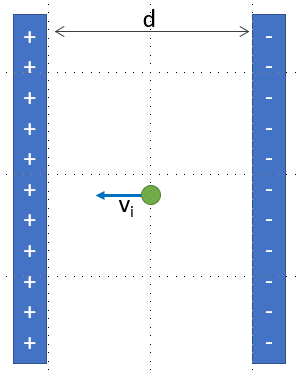
\includegraphics[scale=0.40]{exam1_6.png}
\end{center}
\end{figure}

Assume the distance ($d$) between the plates is $20cm$ and the charge on each plate has a magnitude of $150 \frac{N}{C}$. 



\begin{enumerate}[label=\Alph*]
\item If a proton is at the midpoint between the two plates with initial speed of $10,000 \frac{m}{s}$ in the direction shown, then at what location will the proton change direction due to the electric field?
\item If the proton is replaced with an electron, how does that change the location where the particle changes direction?
\end{enumerate}

\textit{Note: the mass of a proton is $m_p = 1.637 \cdot 10^{-27} kg$ and the mass of a electron is $9.11 \cdot 10^{-31} kg$}. The charge on an electron is $1.602 \cdot 10^{-19} C$.

\textbf{Question 6} (15 pts)

Consider a $475 \mu F$ parallel plate capacitor filled with air. The magnitude of the charge on the plates is $0.114C$ and the separation between the plates is $0.187mm$.

\begin{enumerate}[label=\Alph*]
\item What is the Potential difference between the two plates?
\item What is the area of the plates?
\item What is the magnitude of the Electric Field between the plates?
\item What is the charge density on the plates?
\end{enumerate}

\textbf{Question 7 - Extra Credit} (5pts)
\begin{enumerate}[label=\Alph*]
\item Name one of the two individuals credited with inventing the lightning rod.
\item Draw a lightning rod on top of a building (quality of drawing isn't graded).
\item Describe how and why a lightning rod works.
\end{enumerate}
 

\end{document}
